\section{Test Beam Analysis}

One of the key things in doing a pulse shape analysis using test beam data is the timing information. In the test beam we take two different timing information. The first comes from the QIE chips in the readout modules. The readout modules measure the output charge of the SiPM over 250ns and the information is binned into 10 time samples each 25ns long. The output pulse of the SiPM is about 75ns long so it usually stays confined to 3 or 4 time samples. In addition we also take what is called a Time to Digital Converter (TDC) value. This value stores at what time in the 250ns span the output charge of the SiPM crossed a threshold with a 0.5ns resolution. Since the output charge starts out below this threshold, the TDC value should give the the start of the output pulse of the SiPM. One of the problems with the TDC value is that it could be affected by the amplitude of the output pulse as a high amplitude will cross this threshold earlier. To extract the pulse shape we can do something called a phase scan. In a phase scan we delay starting the taking of data by something less than 25ns. Since the pulse does not come in in time sample 0 we do not loose any of the pulse but simply move parts of the output pulse into different time samples. By doing this we can extract the pulse shape with a resolution much greater than 25ns. 

%\begin{figure}
%\centering
%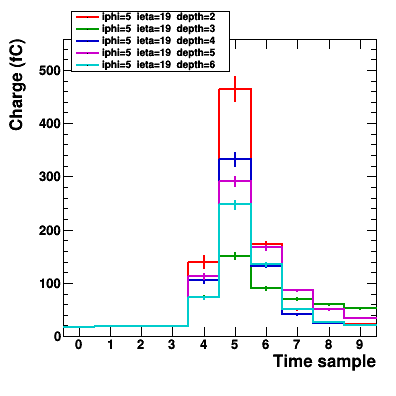
\includegraphics[width=0.6\linewidth]{Figures/PulseShape.png}
%\caption{A histogram of the output pulse of the readout modules binned in 25ns bins.}
%\label{fig:PulSh}
%\end{figure}

There is also the trigger information. This timing information comes from the test beam equipment that signals the back end electronics to store the data from the readout modules. 